\documentclass{style/modernsimplecv}
\usepackage[utf8]{inputenc}
\usepackage[top=2cm, bottom=2cm, outer=0cm, inner=0cm, margin=1cm, a4paper]{geometry}
\usepackage[sfdefault]{AlegreyaSans}
\usepackage{beuron}
\usepackage{setspace}
\usepackage{wallpaper}
\usepackage{mdframed}
\usepackage{enumitem}



\title{Curriculum Vitae}
\author{Paul Brenker}
\date{October 2024}

\pagestyle{empty}
\begin{document}
\thispagestyle{empty}

\tikz[remember picture, overlay] {%
    \node[rectangle, fill=white, anchor=north, minimum width=\paperwidth, minimum height=5cm](header) at (current page.north){};
}
% \begin{minipage}[t]{0.183\textwidth}
%     \vspace{0pt}
%     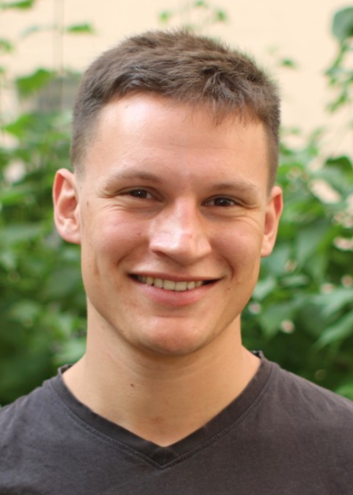
\includegraphics[width=\textwidth]{img/paul.png}\hspace{1em}
% \end{minipage}
% \hfill
\begin{minipage}[t]{0.99\textwidth} % else 80 %
    \vspace{0pt}
    \begin{shaded*}
        \begin{minipage}[t]{0.50\textwidth}
            \vspace{0pt}
            {\par\centering\huge{Paul Brenker}} \\[0.3cm]
            %\faGlobe~ Nationality: German, Work Visa Israel B1\\
            %\faBirthdayCake~ 1996 \\
            \vspace{-3pt}
            \begin{tabular}{l l}
                \faMapMarker~ Tel Aviv, Israel &
                \faPhone~ +972 52 3002843 \\
                \faLink~ \href{https://www.pbrenk.com}{Personal Blog} & 
                \faAt~ \href{mailto:paul.brenker@gmail.com}{paul.brenker@gmail.com}\\
                \faGithub~ \href{https://github.com/paulbrenker}{GitHub} & 
                \faLinkedin~ \href{https://www.linkedin.com/in/paul-brenker}{LinkedIn}\\ 
            \end{tabular}
            \vspace{4pt}
        \end{minipage}\hfill
        \begin{minipage}[t]{0.50\textwidth}
            \vspace{25pt} 
            \faCommentsO~ {Languages:} \\
            \begin{tabular}{l l}
                \textbf{German:} native & \textbf{English:} full proficiency \\
                \textbf{Hebrew:} advanced proficiency & \textbf{Arabic:} basic knowledge \\ 
            \end{tabular}


        \end{minipage}
        \hfill
    \end{shaded*}
\end{minipage}\\
\subsection*{}
\vspace{-3em}
\begin{minipage}{0.99\textwidth}
\section*{Summary}
    \textbf{Backend Software Engineer} with a strong \textbf{Computer Science} background focussed on \textbf{Java Virtual Machine} based Projects. I have valuable experience working for a company that scaled a product from thousands to hundreds of thousands of users working across the \textbf{whole web development stack}. Known for my analytical mindset, persistence, and ability to thrive under pressure I am looking for a dynamic environment that will support my professional growth and technical excellence.
\end{minipage}
\bigskip

    
\begin{minipage}{0.99\textwidth}
    \section*{Experience}
    \begin{tabular}{p{5.2em}| p{0.85\textwidth}}
        \cvevent{2023 - 2024}{SAP LeanIX}{Software Engineer - Student Position}{Bonn, Germany}{
                \item Extended the features of \textbf{key services in the SAP LeanIX} infrastructure.
                \item Worked in an engineering team with a \textbf{heavy focus on collaboration}.
                % \item Built backend REST service for the Architecture Decisions feature (\href{https://app.leanix.net/openapi-explorer?urls.primaryName=Documents}{Documents Service}).
                \item Supported the implementation of one of the \textbf{first agentic AI solution} within the SAP LeanIX product and introduced a qualitative way to test the resulting AI responses verifying 95\% precision.
                \item \textbf{Improved performance of existing backend services by up to 70\%} on large result sets, implementing cursor based pagination in combination with dynamical filtering using the Java Persistence API.
                %\item See a private demo of applied technology stack and coding practices in my own web applications: \href{}{trailmenu}, \href{}{trailmenu-frontend}
                }
            {img/leanix_logo.jpg}\\

        \cvevent{2023}{LeanIX}{Intern}{Bonn, Germany}{
                \item \textbf{Evaluated API linting tools for the services in the LeanIX infrastructure}. For that I compared different tools, evaluated pros and cons, and implemented a full set of rules validating compliance to company's REST guidelines.
            }
            {img/leanix_logo_old.jpg}\\

        \cvevent{2021 - 2023}{University of Bonn}{IT Support Student Assistant}{Bonn, Germany}{
                \item Maintenance and Acquisition of IT \textbf{hardware and software} such as network devices, printers and personal computers.
            }
            {img/uni_bonn_logo.png}\\

        % \cvevent{2017 - 2018}{Academy of Sciences and Humanities}{Student Assistant}{Berlin, Germany}{
        %     \vspace{-.4cm}
        %     \begin{itemize}[leftmargin=.3cm]
        %         \setlength\itemsep{-.1em}
        %         % \item Worked in the Digital Humanities department on the \href{https://corpuscoranicum.de/en}{Corpus Coranicum} project.
        %         % \item Transcribed and annotated ancient Hebrew and Arabic texts using DIN 31635 transliteration.
        %         \item Developed XML schemes for auto referencing to external resources via Zotero and for internal cross-referencing in project database.
        %     \end{itemize}
        %     }
        %     {img/bbaw_logo.jpg}\\    
    \end{tabular}

    \section*{Skills}
    \begin{tabular}{p{5.2em}| p{0.85\textwidth}}
        \cvskills{Cloud}{
            \textbf{AWS (currently studying for Certified Developer Associate)}, 
            Azure, Kubernetes, \textbf{Docker}}\\
        %\cvskills{Containers}{Docker}\\
        \cvskills{CI/CD}{\textbf{GitHub Actions}, Jenkins}\\
        \cvskills{VC}{Git (\textbf{GitHub}, GitLab)}\\
        \cvskills{OS}{\textbf{Linux} Server \& Desktop}\\
        \cvskills{Observability}{
            IBM Instana, 
            Grafana}\\
        \cvskills{Languages}{
            \textbf{Java \& Kotlin} for Backend,
            \textbf{Typescript} for Frontend,
            \textbf{Python} for Data Science}\\
        \cvskills{Frameworks}{
            \textbf{Spring Boot} including \textbf{Spring Security} and \textbf{Spring Data JPA}, 
            \textbf{REST APIs} with OpenAPI,
            \textbf{Angular}}\\
        \cvskills{Testing}{JUnit5, MockK, Jest, Selenium}\\
        %\cvskills{Libraries}{Numpy, Pandas, SkLearn}\\
        \cvskills{Databases}{
            \textbf{PostgreSQL}, 
            Oracle}\\
        \cvskills{Data Science}{
            Statistical Methods, 
            Natural Language Processing, 
            \textbf{Machine Learning}}\\
        \cvskills{Methods}{
            \textbf{Technical Documentation}, 
            Software Architecture, 
            \textbf{TDD}, 
            Relational DB Design, 
            Agile, 
            Microservices}\\
    \end{tabular} 
    

    \section*{Education}
    \begin{tabular}{p{5.2em}| p{0.85\textwidth}}
        \cvevent{2019 - 2024}{Bonn-Rhein-Sieg University of Applied Sciences (H-BRS)}{B.Sc. Computer Science}{Bonn, Germany}{
                \item \textbf{Computer Science} degree with a final grade of 1.6 GPA (German) (\textbf{$\equiv$ 92\% Israeli}) within the \textbf{best 10 \%} of graduates.
                \item Specialized in \textbf{Bioinformatics and Data Science} where I did multiple applied projects. (E.g. \href{https://github.com/paulbrenker/decision-tsp}{see here})
                \item For my Thesis I chose the topic: \textbf{Relevance of OpenAPI Linter Rules} for Specification Quality. (\href{https://github.com/paulbrenker/thesis}{Thesis Repo})
                \item Deutschlandstipendium - \textbf{Scholarship for ambitious and talented students}.
            }
            {img/hbrs_logo.jpg} \\
            
        \cvevent{2015 - 2019}{Freie Universität zu Berlin}{B.A. Linguistics}{Berlin, Germany}{
                \item Focused on \textbf{Middle Eastern languages} including \textbf{Hebrew}, Arabic, Amharic and Aramaic.
                \item PROMOS -  Scholarship for a Hebrew summer school at the \textbf{Ben Gurion University of the Negev}.
                \item DAAD Scholarship for \textbf{intensive Arabic language} courses at the German Jordanian University in Amman, Jordan.
                \item Thesis was written about gender-specific variations in the Arabic dialect of Amman, Jordan. 
            }
            {img/fu_logo.png} \\
    \end{tabular}
\end{minipage}
    % \begin{minipage}{0.99\textwidth}
    %     \section*{Scholarships}
    %     \begin{tabular}{>{\bfseries}p{0.12\textwidth} >{}p{0.7\textwidth}}
    %         2023 & Deutschlandstipendium - Scholarship for ambitious and talented students.\\
    %         2018 & DAAD Scholarship for intensive Arabic language courses at the German Jordanian University in Amman, Jordan.\\
    %         2018 & PROMOS -  Scholarship for a Hebrew summer school at the Ben Gurion University of the Negev.\\
    %     \end{tabular}
    % \end{minipage}\hfill



    % \bigskip
    % \begin{minipage}[t]
    %     \section*{Volunteering}
    %     \begin{tabular}{>{\bfseries}p{0.12\textwidth} >{}p{0.7\textwidth}}
    %         2014 & After graduating from high school I volunteered for nine months in Kibbutz Ein Hashlosha in Israel. During my time I worked mostly in agriculture and landscaping but also in the local garage where I helped to maintain the vehicles of the Kibbutz. \\
    %     \end{tabular}
    %     \bigskip
    %     \section*{Hobbies}
    %     \begin{tabular}{>{\bfseries}p{0.12\textwidth} >{}p{0.7\textwidth}}
    %         Rowing  & I row since I am ten years old and participated in countless competitions including the German national sprint league. \\
    %         Cycling & I love to ride bicycles not just for sport but also in the everyday for a sustainable and balanced life.
    %     \end{tabular}
    % \end{minipage}

\end{document}